%20/02 - Ana González Marcos
\chapter{Aplicación de algoritmos a problemas bioinformáticos}
La búsqueda de motivos se realiza mediante búsqueda exhaustiva, algoritmos codiciosos o algoritmos aleatorios. Los algoritmos de programación dinámica se emplean para los alineamientos. Un motivo es una secuencia específica y corta que aparecen frecuentemente en una región del ADN o secuencia proteica. Representa una región conservada en secuencias que suelen tener significado biológico. 

\section{Búsqueda exhaustiva}
La búsqueda exhaustiva es la única búsqueda "de verdad" que da una solución determinista exacta. También se conoce como búsqueda por fuerza bruta. El algoritmo examina todas las posibles alternativas para encontrar una solución óptima. El tiempo de cómputo es muy alto, pese a que requiera de poco esfuerzo en su diseño. Como las secuencias biológicas son muy largas, este tipo de búsquedas es inviable. 
En el patrón se busca encontrar un consenso que se puede representar gráficamente en logos. 

Una posible aplicación es la búsqueda de un patrón de x nucleótidos (x-mer) sin mutaciones. También se pueden incorporar un par de mutaciones y generar un consenso. Con esto se calcula el perfil y se ve cuántos nucleótidos caen en cada posición. Se busca el perfil que, aun con mutaciones, da un motivo consenso. 

El consenso es un motivo ancestro del cual surgen los motivos mutados. Para calcular la medida que indique lo buen consenso que es un motivo, se tiene en cuenta la homología, es decir, la similitud debida a un ancestro común. La distancia entre un motivo real y la secuencia de consenso suele ser menor que la de dos motivos reales. Necesitamos introducir una función de puntuación para comparar diferentes conjeturas (consenso) y elegir la «mejor». 
$$Score(s, DNA) = \sum^l_{i = 1} \max_{k \in A T G C} count(k, i)$$

Se busca a lo largo de todas las cadenas, desde la primera posición el tamaño del l-mer. En definitiva, el algoritmo es:
\begin{lstlisting}
BruteForceMotifSearch(DNA, t, n, l)
bestScore = 0
for each s=(s1, s2, ..., st) from (1, 1 ... 1) to (n-l + 1, ..., n-l + 1)
	if Score(s, DNA) > bestScore
		bestScore = score(s, DNA)
		bestMotif = (s1, s2, ... st)
return bestMotif
\end{lstlisting}

Como esta búsqueda es exhaustiva, para $(n - l + 1)$ posiciones en t secuencias, se buscan $(n - l + 1)^t$ sets de posiciones iniciales. Para cada posición inicial, la función de puntuación hace $l$ operaciones, de forma que la complejidad es:
$$l \cdot (n - l + 1)^t \rightarrow O(l \cdot n^t)$$
De esta forma, hay veces en las que no es posible hacer este cálculo.

\subsection{Median String}
El median string es la alternativa a la búsqueda exhaustiva. En este caso se busca en las secuencias un patrón. No se utiliza la puntuación de antes, si no que utiliza la distancia de Hamming. La distancia de Hamming entre dos mer se define como el número de nucleótidos distintos entre ellos. 
$$d_H(AAAAAA, ACAAAC) = 2$$
$$d_H(v, s) = \sum^t_{i = 1} d_H(v, s_i)$$
Antes se buscaba la puntuación máxima, pero ahora buscamos la distancia mínima. 

\begin{lstlisting}
MedianStringSearch(DNA, t, n, l)
bestWord = AAAAA...A
bestDistance = infinity
for each l-mer v from AAA...A to TTT...T
	if TotalDistance(v, DNA) < bestDistance:
		bestDistance = TotalDistance(v, DNA)
		bestWord = v
return bestWord
\end{lstlisting}

La búsqueda de motivos es un problema de maximización, mientras que la cadena mediana es un problema de minimización. Sin embargo, el problema de la Búsqueda de Motivos y el de la Cadena Mediana son computacionalmente equivalentes. Hay que demostrar que minimizar TotalDistance es equivalente a maximizar la puntuación.

Con este algoritmo, la complejidad es de $4^l$. El coste es considerablemente más bajo que en la búsqueda exhaustiva, ya que el tamaño del mer es más pequeño que el tamaño de la secuencia. Por tanto, reformular un problema puede ayudar a disminuir la complejidad computacional. 

%25/02 - Ana
\section{Algoritmo codicioso}
Un algoritmo codicioso es un algoritmo que siempre toma la mejor solución inmediata, o local, mientras encuentra una respuesta.
Los algoritmos codiciosos:
\begin{itemize}
\item a menudo devuelven resultados subóptimos, pero tardan poco en hacerlo.
\item seleccionan la alternativa «más atractiva» en cada iteración.
\item suelen ser heurísticas rápidas que cambian precisión por velocidad para encontrar una solución aproximada/subóptima.
\end{itemize}

En este caso, se utiliza la entropía como medida. Es una medida probabilística que se suele definir como $\int -p \log (p)$. Está la entropía sobre todos los nucleótidos se correspondería a $- \sum p \cdot \log_2(p)$. Esto se utiliza para calcular los logos. Motif logo es un diagrama para visualizar la conservación de motivos que consiste en una pila de letras en cada posición. La altura total de cada columna se basa en el contenido informativo de la columna, que se define como $2 - H_i(p_A, p_C, p_G, p_T)$. Cuanto menor es la entropía, mayor es el contenido de información, lo que significa que las columnas altas del logotipo del motivo están muy conservadas. 

La probabilidad del l-mer es la probabilidad de que un l-mer a fuese creado por el perfil P:
$$p(a|P) = \Pi^l_{k=1} P_{a_{i,k}}$$ 
donde $P_{a_{i,k}}$ es la probabilidad de la letra $a_i$ en la posición $k$, distribuida independientemente e idénticamente. 

\begin{lstlisting}
GreedyMotifSearch(DNA, k, t)
BestMotifs = primer k-mer de cada string de ADN
for each k-mer Motif in the first string in DNA do
	Motif1 = Motif
	for i = 2 to t do
		form Profile from Motif1, ..., Motif i-1
		Motif i = profile-most probable k-mer in the ith string in DNA
	Motifs = Motif i, ..., Motif t
	if Score(Motif) > Score (BestMotif) then
		BestMotifs = Motifs
return BestMotifs
\end{lstlisting}

Primero, se inicializa una matriz de motivos con los primeros -lmers de cada secuencia de ADN. Después se va comparando el l-mer de la primera secuencia con la siguiente secuencia, calculando el mejor motivo, el cual se añade a una nueva lista. Así se recorren las distintas secuencias. Tras obtener la lista de los motivos (uno por cada secuencia), se obtiene el consenso. Éste se puntúa y se compara con la puntuación de la matriz inicializada, quedándonos con la matriz que tenga una puntuación mayor. A continuación se mueve el primer l-mer un nucleótido y repetir todo este proceso.

Para evitar obtener resultados de 0, se utiliza la regla de sucesión de Laplace, sumando 1 a todos los valores de contaje para computar las probabilidades mediante pseudo-counts. De esta forma, se obtiene la matriz del perfil. 

En cuanto al tiempo del cómputo, como tenemos una matriz $t \times n$ de ADN y una longitud del patrón $l$, el tiempo de ejecución es $O(n^2 \cdot l \cdot t)$, lo cual es mejor que el algoritmo de fuerza bruta. No obstante, es restrictivo, por lo que podemos no encontrar los mejores motivos. Cambiando el orden de las secuencias, el resultado va a ser distinto, afectando significativamente el rumbo que tomará el análisis. 

\section{Algoritmos randomizados}
Los algoritmos aleatorios toman decisiones aleatorias en lugar de deterministas. Estos algoritmos se utilizan en situaciones en las que no se conoce ningún algoritmo polinómico correcto. Seleccionan aleatoriamente posibles ubicaciones y encuentran una forma de cambiar codiciosamente esas ubicaciones hasta que hayamos convergido al motivo oculto.

\begin{lstlisting}
RandomizedMotifSearch(DNA, l, t)
Randomly select l-mers Motifs = (Motif1, ... Motift) in each string from DNA
BestMotifs = Motifs
while forever
	Profile = PROFILE(Motifs)
	Motifs = MOTIF(Profile, DNA)
	if Score(Motifs) > Score(BestMotifs)
		BestMotifs = Motifs
	else
		return BestMotifs
\end{lstlisting}

Este algoritmo se detiene tras un número de iteraciones que le demos, o cuando el perfil apenas se modifique tras más iteraciones. El algoritmo se ejecuta muchas veces, cada una de ellas con nuevos l-mers inicializados, y con la colección de los motivos con mayor puntuación se obtiene el consenso. 

\subsection{Gibbs Sampling}
RandomizedMotifSearch puede cambiar todas las cadenas $t$ en Motifs en una única iteración. Puede sondear imprudentemente, y algunos motivos correctos pueden ser descartados en la siguiente iteración.

GibbsSampler es un algoritmo iterativo más cauteloso que descarta un único $l$-mers del conjunto actual de motivos en cada iteración y decide conservarlo o sustituirlo por uno nuevo. Los pasos son:
\begin{enumerate}
\item Elegir aleatoriamente las posiciones iniciales de l-mers para cada secuencia.
\item Elegir al azar una de las secuencias $t$
\item Crear un perfil $P$ (consenso) a partir de las otras secuencias ($t - 1$)
\item Para cada posición de la secuencia eliminada, se calcula la probabilidad de que el $l$-mer que comienza en esa posición haya sido generado por $P$.
\item Elegir al azar una nueva posición inicial para la secuencia eliminada basándose en las probabilidades calculadas en el paso anterior.
\end{enumerate}

Este proceso se itera hasta dar con la solución, es decir, que la puntuación no mejore más. 
GibbsSampler funciona bien en muchos casos. Dado que GibbsSampler explora sólo un pequeño subconjunto de soluciones, puede «atascarse» en un óptimo local. Al igual que RandomizedMotifSearch, debe ejecutarse varias veces con la esperanza de que una de estas ejecuciones produzca los motivos con mejor puntuación.

Estos algoritmos aleatorizados funcionan porque el ADN no es del todo aleatorio, conteniendo motivos reguladores que permiten un control preciso sobre la expresión genética. Estos motivos resultan en un perfil esperado sesgado.

%27/02
\section{Algoritmo divide-y-vencerás}
En estos algoritmos, el problema se divide en subproblemas, conquistándolos de forma recursiva. Si los subproblemas son lo suficientemente pequeños, se resuelven de forma bruta. Las soluciones de los subproblemas se deben combinar en una solución para el problema original, siendo esto lo complicado. Un algoritmo de divide y vencerás hace más trabajo del necesario, resolviendo repetidamente los subproblemas comunes. 

\section{Programación dinámica}
La programación dinámica se basa en la premisa de calcular primero las soluciones a subproblemas más pequeños y utilizarlas después para resolver problemas sucesivamente más grandes hasta obtener la respuesta. La programación dinámica se utiliza cuando se podría recurrir a la recursividad, pero sería ineficaz porque resolvería repetidamente los mismos subproblemas. Se toma un problema que podría resolverse recursivamente de arriba abajo y, en su lugar, se resuelve iterativamente de abajo arriba. Los resultados intermedios se almacenan en una tabla para su uso posterior; de lo contrario, se acabarían calculando repetidamente, lo que constituye un algoritmo ineficaz.

Por ejemplo, la programación dinámica se utiliza para ver la similitud entre genes. El alineamiento de secuencias es esencial para filogenia, análisis genómico, predicción de genes, estructura proteica, estructura de ARN secundario, búsqueda en bases de datos, etc. Si los alineamientos son erróneos, todos los resultados basados en los alineamientos están mal.

En el alineamiento de secuencias se distingue el alineamiento por pares, donde se alinean dos secuencias, del alineamiento múltiple, donde se utilizan más de dos secuencias. 

\subsection{Problema de la subsecuencia común más larga}
Los biólogos que encuentran una nueva secuencia genética suelen querer saber con qué otras secuencias es más parecida. Encontrar una subsecuencia es una forma de calcular el grado de similitud entre dos secuencias: cuanto más larga es la subsecuencia, más similares son. Los caracteres de una subsecuencia, a diferencia de los de una subcadena, no tienen por qué ser contiguos.

\subsection{Matriz de sustitución}
El problema del ADN es que puede mutar: mutación puntual de un nucleótido, inserción o deleción. Encontrar la similitud del ADN es importante, ya que secuencias similares pueden tener funciones similares. Uno de los algoritmos más ampliamente utilizados es BLAST. 

La matriz de puntuación de sustitución es una matriz bidimensional con valores de puntuación que describen la probabilidad de que un aminoácido o nucleótido haya sido reemplazado durante la evolución de la secuencia. Se pueden penalizar la apertura de huecos y la mutación puntual, creando una matriz ponderada. Se da una puntuación positiva a los pares de caracteres idénticos o similares y una puntuación negativa a los diferentes. Esta puntuación se basa en las frecuencias observadas de tales ocurrencias en alineaciones de ADN/proteínas relacionadas evolutivamente.

El parámetro más crítico en la comparación de secuencias es la elección de una matriz de puntuación/sustitución. Para una evolución reciente, se suele utilizar una matriz de identidad, ya que se espera que las secuencias no hayan divergido mucho. Para una evolución antigua, la matriz converge a un modelo aleatorio. En bioinformática hay varias matrices: PAM, BLOSUM, Gonnet, JTT.

\subsection{Matrices de puntuación}
\paragraph{PAM}
PAM viene de Point Accepted Mutation. Contiene la probabilidad derivada empíricamente de que se acepte una sustitución, basada en proteínas estrechamente relacionadas. Los números PAM más altos corresponden a una mayor distancia evolutiva. Cuando dos secuencias tienen una diferencia de 1 PAM, significa que una secuencia se puede transformar en la otra con una media de mutaciones puntuales de un 1\% (una mutación por cada 100 aminoácidos).

\paragraph{BLOSUM}
BLOSUM viene de Blocks Substitution Matrix. Es otra matriz derivada empíricamente, basada en proteínas relacionadas a mayor distancia. Los números BLOSUM más bajos corresponden a una mayor distancia evolutiva.

La comparación entre PAM y BLOSUM, a un nivel comparable de sustituciones, indica que los dos tipos de matrices producen resultados similares

\subsection{Needleman-Wunsch - alineamiento global}
Este método realiza un alineamiento global entre dos secuencias. Se inicializa en 0, y se rellena la matriz con el valor máximo entre la mutación puntual o el hueco (ya sea en una secuencia o en la otra) mediante la matriz de puntuación. 

\begin{figure}[h]
\centering
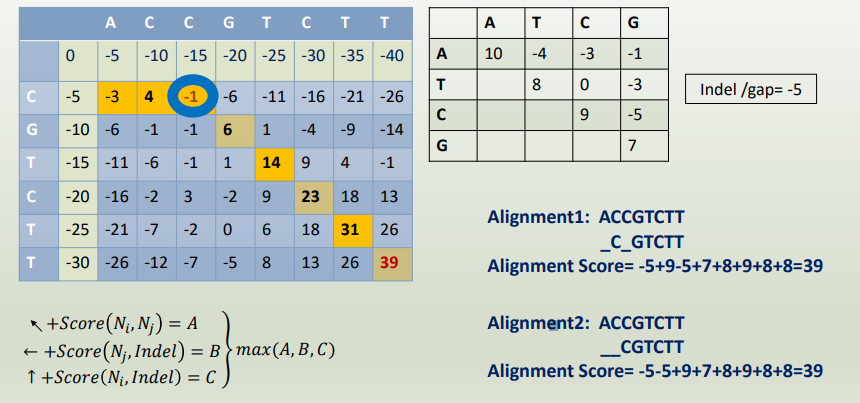
\includegraphics[width = 0.8\textwidth]{figs/needleman-wunsch.png}
\end{figure}

Una vez calculada la matriz F, la esquina inferior derecha de la matriz es la puntuación máxima de cualquier alineación. Para calcular qué alineación da realmente esta puntuación, se puede empezar por la celda inferior derecha y comparar el valor con las tres fuentes posibles (Opción1, Opción2 y Opción3) para ver de cuál procede.
\begin{itemize}
\item Si es la opción 1, entonces las dos secuencias están alineadas.
\item Si es la opción 2, entonces la primera secuencia está alineada con un hueco.
\item Si es la opción 3, entonces la segunda secuencia está alineada con un hueco.
\end{itemize}

El alineamiento global suele utilizarse para alinear secuencias que tienen aproximadamente la misma longitud y que ya se sabe que están relacionadas.

\subsection{Smith-Waterman - alineamiento local}
En este caso, se busca la mejor puntuación de los alineamientos de regiones de secuencias. De esta forma, se encuentran segmentos conservados, en lugar de alinear la secuencia completa. La diferencia con Needleman-Wunsch es la posibilidad de coger 0 como posibilidad a la hora de rellenar la matriz.

\begin{figure}[h]
\centering
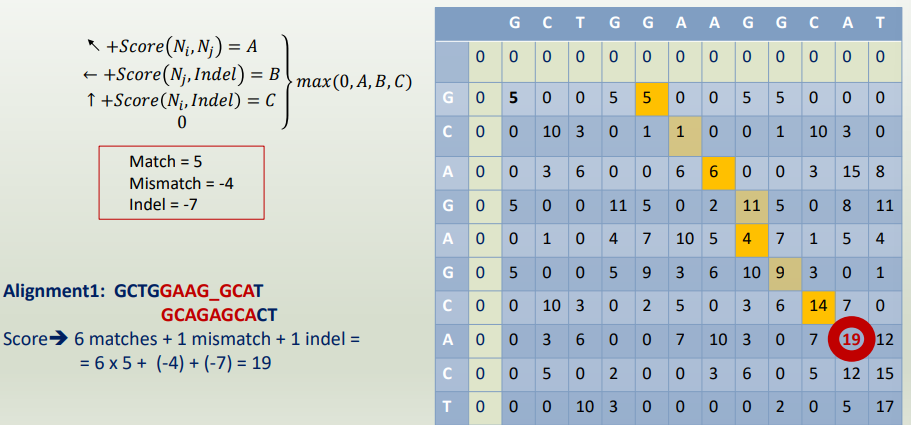
\includegraphics[width = 0.8\textwidth]{figs/smith-waterman.png}
\end{figure}

Tanto el algoritmo de Needleman-Wunsch como el de Smith-Waterman utilizan los conceptos de matriz de sustitución/puntuación, función de penalización por hueco y proceso de rastreo. 

\begin{table}[h]
\begin{mdframed}[backgroundcolor=black!10]
\textbf{Ejercicio:} encuentra el mejor alineamiento local entre TCAGTTGCC y AGGTTG con +1 para match, -2 para mistmatch y -2 para gap.

\begin{tabular}{c c c c c c c c c c c}
&&T&C&A&G&T&T&G&C&C\\
&0&0&0&0&0&0&0&0&0&0\\
A &0 &0&0&1&0&0&0&0&0&0\\
G &0 &0&0&0&2&0&0&0&0&0\\ 
G &0 &0&0&0&3&1&0&2&0&0\\ 
T &0 &1&0&0&1&4&1&3&1&0\\ 
T &0 &2&0&0&0&5&5&6&2&0\\ 
G &0 &0&0&0&2&1&3&6&5&3\\ 
\end{tabular}

Por tanto, la parte común es GTTG.

\textbf{Ejercicio:} lo mismo que antes, pero para el mejor alineamiento global.
\begin{tabular}{c c c c c c c c c c c}
&&T&C&A&G&T&T&G&C&C\\
&0&-2&-4&-6&-8&-10&-12&-14&-16&-18\\
A &-2 &-2&-4&-3&-5&-7&-9&-11&-13&-15\\
G &-4 &-4&-6&-5&-2&-4&-6&-8&-10&-12\\ 
G &-6 &-6&-8&-7&-4&-3&-5&-5&-7&-9\\ 
T &-8 &-4&-6&-7&-5&-2&-2&-4&-6&-8\\ 
T &-10 &-6&-6&-8&-6&-3&-1&-3&-5&-7\\ 
G &-12&-8&-8&-8&-5&-5&-3&0&-2&-4\\ 
\end{tabular}
Por tanto, el resultado es:\\
TCAGTTGCC\\
AG-GTTG
\end{mdframed}
\end{table}

%04/03 - Ana
\section{Búsqueda en bases de datos}
El tiempo de búsqueda en grandes bases de datos es una consideración importante, y se hace necesario equilibrar la velocidad y la sensibilidad de la búsqueda. Los métodos exhaustivos, como Needleman-Wunsch y Smith-Waterman, suelen garantizar una respuesta óptima, pero tardan demasiado en comparar una secuencia con una base de datos. En un intento de ganar velocidad con una pérdida aceptable de sensibilidad, se han derivado métodos aproximados a partir de estos algoritmos.

\subsection{Métodos heurísticos}
Los métodos heurísticos para buscar en una base de datos son:
\begin{itemize}
\item FastA: Primer algoritmo rápido de búsqueda de secuencias para comparar una secuencia de consulta con una base de datos
\item BLAST: Es una mejora de FastA en cuanto a velocidad de búsqueda, facilidad de uso, rigor estadístico y sensibilidad.
\end{itemize}

Tanto FASTA como BLAST buscan similitud local entre secuencias.

\subsubsection{FastA}
FastA es un algoritmo de varios pasos para el alineamiento de secuencias. Primero se buscan regiones de dos secuencias que parezcan prometedoras, es decir, que tengan algún grado de similitud. Después se computa el alineamiento local usando programación dinámica en estas regiones. Si simplemente se comparan dos secuencias cualesquiera para ver si son homólogas, Smith-Waterman sería el método a elegir. Las características de FastA son:
\begin{itemize}
\item Alineamiento local: intenta encontrar parches de similitud regional, en lugar de tratar de encontrar el mejor alineamiento entre toda la secuencia query y las secuencias de la base de datos. 
\item Alineamiento con gaps: los alineamientos generados pueden contener huecos.
\item Rapidez: es un método heurístico, pudiendo perder coincidencias. Así, no hay garantía de encontrar el mejor alineamiento. Utiliza una estrategia que sacrifica la sensibilidad completa para ganar velocidad.
\end{itemize}

La programación dinámica calcula la puntuación en un montón de zonas inútiles para encontrar secuencias subóptimas. Se buscan secuencias cortas en las que haya matches. Normalmente, en el ADN se busca con una longitud de 6 nucleótidos y para proteínas 2 aminoácidos. 
Los pasos del algoritmo son:
\begin{enumerate}
\item Identificar k-meros comunes entre las secuencias I y J.

Los k-meros comunes se representan en un dot matrix. Cada elemento tiene un punto si el k-mero que inicia en esa posición coincide entre ambas secuencias.
\begin{figure}[h]
\centering
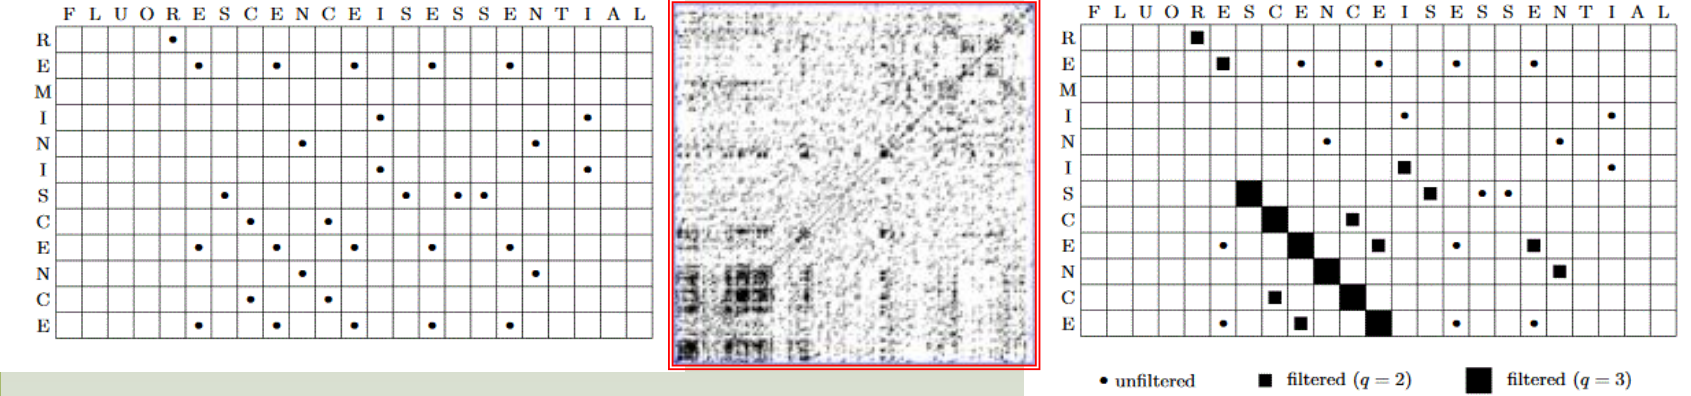
\includegraphics[width = \textwidth]{figs/dotmatrix.png}
\end{figure}

\item Puntuar la diagonal con los matches de los k-meros, identificando las 10 mejores diagonales.

Sobre el ejemplo, la matriz dot serían los puntos. Se coge como referencia la diagonal principal. Sobre ella, se realizan los desplazamientos positivos (hacia abajo) y negativos (hacia arriba). Los matches que se encuentran son los puntos que caen en las celdas de la diagonal. 
\begin{figure}[h]
\centering
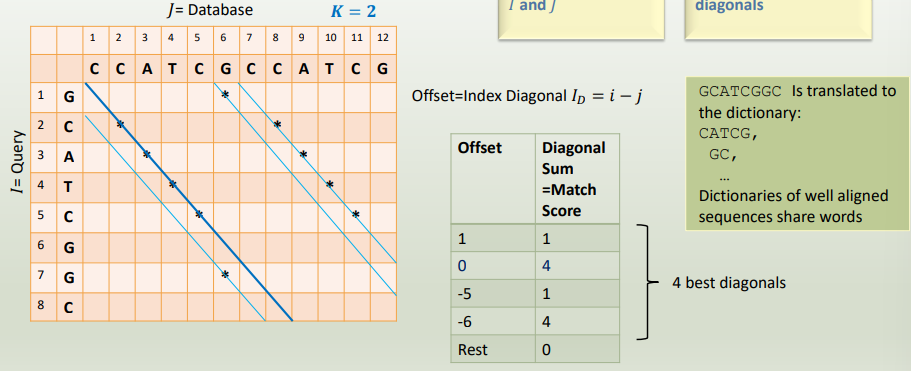
\includegraphics[width = \textwidth]{figs/diagonal-sums.png}
\end{figure}

\item Volver a puntuar regiones iniciales con una matriz de sustitución (PAM o BLOSUM).

Cada diagonal de puntuación alta elegida en el paso anterior se vuelve a puntuar según una matriz de puntuación (es decir, PAM). Esto se hace para encontrar subregiones con identidades más cortas que k. Los extremos de la diagonal que no coinciden se recortan. El parámetro más crítico en la comparación de secuencias es la elección de una matriz de puntuación.

\item Unir las regiones utilizando gaps, penalizándolos
\begin{figure}[h]
\centering
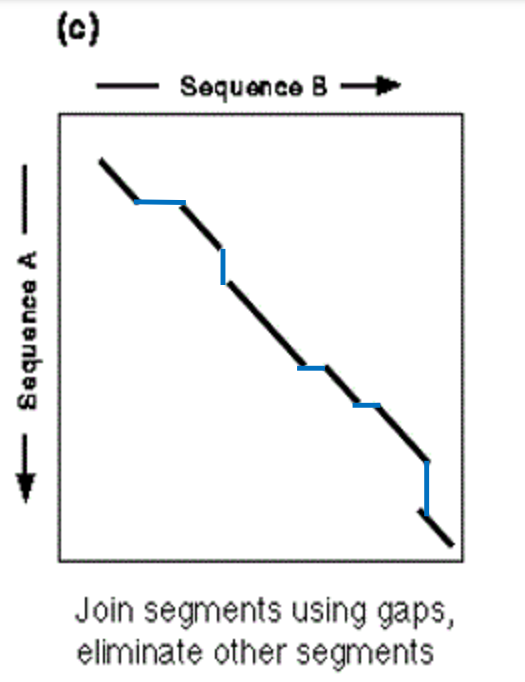
\includegraphics[width = 0.3\textwidth]{figs/join-segments.png}
\end{figure}

\item Utilizar programación dinámica para encontrar un alineamiento final.
\begin{figure}[h]
\centering
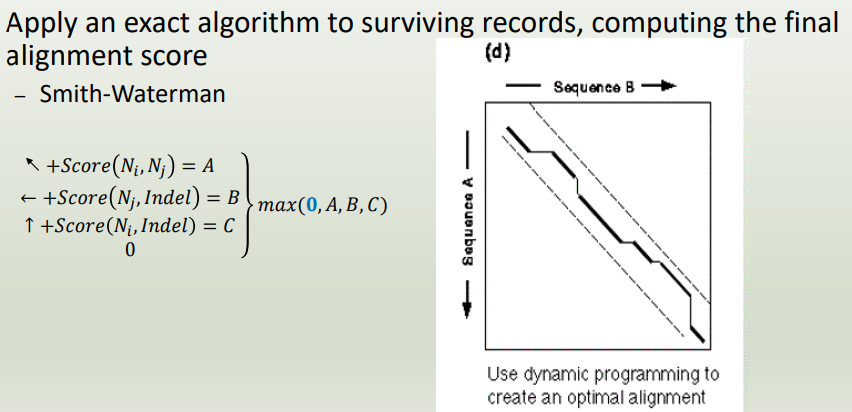
\includegraphics[width = 0.3\textwidth]{figs/final-fasta.png}
\end{figure}
\end{enumerate}

\paragraph{Evaluar la significancia del alineamiento}
Cuando se detecta similitud entre secuencias, hay dos posibilidades: que se deba al azar o debido a la evolución de un ancestro común (y por tanto una función similar). Por ello, se busca obtener una medida universal para inferir homología. ¿Qué diferencia hay entre el resultado de una coincidencia aleatoria y el de una coincidencia entre secuencias no relacionadas? Dado un conjunto de secuencias no relacionadas con la consulta (o un conjunto de secuencias aleatorias), ¿cuál es la probabilidad de encontrar una coincidencia con la misma puntuación de alineación por azar?
En una típica búsqueda actual en bases de datos, una proteína de longitud 250 podría ser comparada con una base de datos de proteínas de 50.000.000 de residuos totales.

Hay distintas medidas para ver la significancia estadística:
\begin{itemize}
\item \textbf{p-valor:} la probabilidad de que al menos una secuencia produzca la misma puntuación por azar. $P_{value} (S) = P(x \geq S)$, siendo S la puntuación y x la secuencia.

\item \textbf{E-valor:} número esperado de secuencias que producirán la misma o mejor puntuación por azar. Es la corrección de los p-valores para pruebas múltiples: $E_{value}(S) = P_{value} \cdot length.database \cdot length.query$

El valor E disminuye exponencialmente a medida que aumenta la puntuación (S) que se asigna a una coincidencia entre dos secuencias. Esto se debe a que, como la secuencia es más larga, hay más probabilidad de que se den matches. El valor E depende del tamaño de la base de datos (N) y del sistema de puntuación utilizado (es decir, PAM150, BLOSUM62). El valor E (asociado a una puntuación S) es el número de alineamientos distintos, con una puntuación equivalente o mejor que S, que se espera que se produzcan en una búsqueda en una base de datos por azar. Cuanto menor sea el valor E, más significativa será la puntuación. Como norma general:
\begin{itemize}
\item $Escore < 10^{-6}$: estadísticamente significativo
\item $10^{-6} < Escore < 10^{-3}$: se debe revisar.
\item $10^{-3} < Escore$: no significativo.
\end{itemize}

$$E = k \cdot m \cdot N |cdot e^{-\lambda S}$$
siendo:
\begin{itemize}
\item m: tamaño de la secuencia query
\item N: tamaño de la base de datos
\item k: constante estadística
\item $\lambda$: constante para ajustar la matriz de puntuación
\item S: puntuación de un high-scoring segment pair
\end{itemize}

\item \textbf{z-score:} mide cuántas desviaciones estándar hay por encima de la media de la distribución de la puntuación.
$$Z_{score} = \frac{S - \mu_S}{\sigma_S}$$

Se generan alineamientos aleatorios y se calcula su puntuación. Con eso, se calcula la media y la desviación estándar de las puntuaciones aleatorias, de forma que después se pueda calcular la desviación de la puntuación actual con la media de las puntuaciones aleatorias. La probabilidad de un z-score se denomina como e-valor.
\end{itemize}

\paragraph{Ejemplo: Retinoblastoma (RBP) vs $\beta$-lactoglobulina}
La segunda secuencia se aleatoriza 100 veces, permutando aleatoriamente («Barajando») las posiciones que ocupan los aminoácidos (manteniendo por tanto la longitud de la secuencia y la composición de aminoácidos). Cada secuencia aleatoria se alinea con la primera y se obtienen 100 puntuaciones «aleatorias». Es de esperar que la puntuación real sea mucho mayor que las 100 puntuaciones «aleatorias».
\begin{figure}[h]
\centering
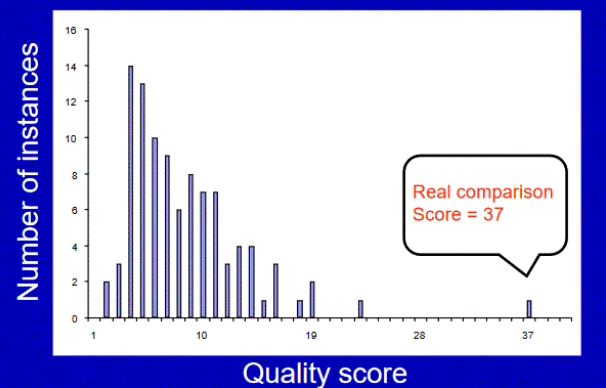
\includegraphics[width = 0.5\textwidth]{figs/shuffling.png}
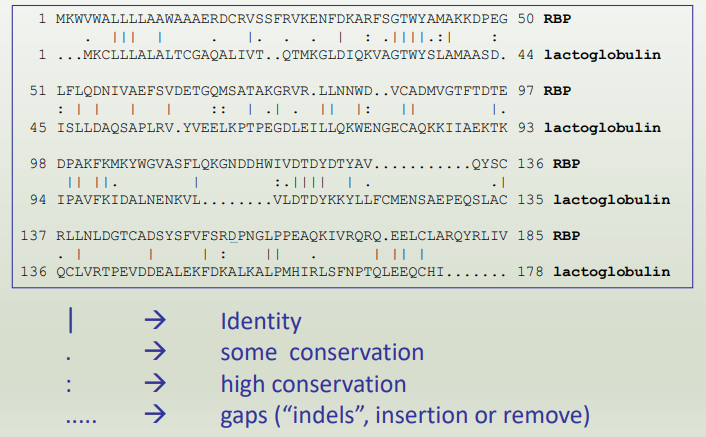
\includegraphics[width = 0.6\textwidth]{figs/alignment-ex.png}
\end{figure}

%06/03 - Ana
\subsubsection{BLAST}
El programa Basic Local Alignment Search Tool (BLAST) se utiliza ampliamente para alinear secuencias. El concepto básico es que:
\begin{itemize}
\item cuanto mayor sea el número de segmentos similares entre dos secuencias, y
\item cuanto mayor sea la longitud de los segmentos similares, menos diferentes son las secuencias y, por tanto, más relacionadas genéticamente (homólogas) es probable que estén
\end{itemize}

BLAST no garantiza el alineamiento óptimo al ser un método heurístico. Tiene un preprocesamiento en el que se crea una tabla de búsqueda de todos los k-meros. Los pasos son:
\begin{enumerate}
\item \textbf{Identificar semillas:} encuentra todos los substrings de longitud k en la secuencia de búsqueda que también está en la base de datos mediante la tabla de búsqueda.
\item \textbf{Extensión de semilla:} cada semilla se extiende hacia ambos lados hasta que la puntuación de alineamiento caiga por debajo de un umbral. Hay dos formas de extensión: sin huecos (solo se extiende con match o missmatch) o con huecos (se permite extender con match, missmatch o un número limitado de gaps).
\item \textbf{Registrar} todos los alineamientos locales que superen un determinado umbral estadístico. 
\item \textbf{Clasificar y ordenar} todos los alineamientos locales en orden ascendente del E-valor.
\end{enumerate}

\begin{figure}[h]
\centering
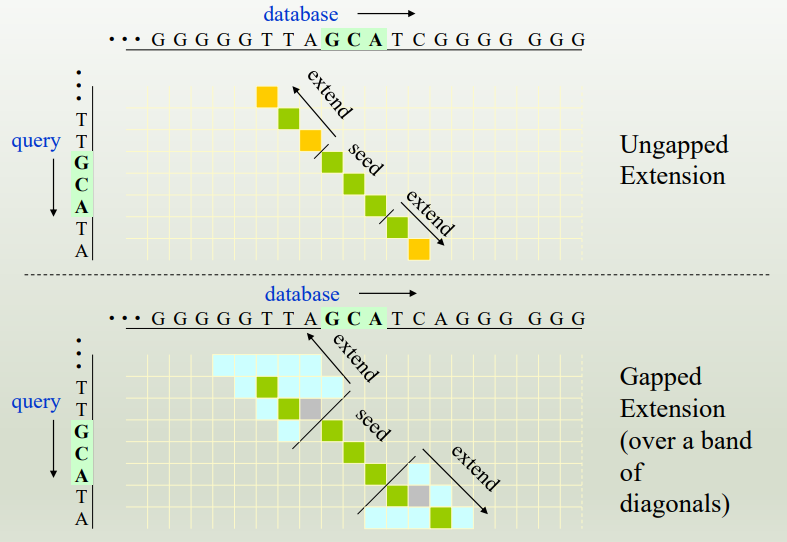
\includegraphics[width = 0.8\textwidth]{figs/blast.png}
\end{figure}

Si se tratara simplemente de comparar dos secuencias cualesquiera para ver si son homólogas, Smith-Waterman sería el método a elegir. FASTA y BLAST se utilizan en búsquedas de homólogos en grandes bases de datos: «Tengo una proteína/secuencia y quiero preguntar si está relacionada con algo de lo que se sepa algo». BLAST y FASTA son tan rápidos en parte porque empiezan buscando «palabras» cortas que coincidan exactamente y construyen un alineamiento más largo a partir de estas palabras. Como contrapartida a la ventaja de la velocidad, es posible que se pasen por alto algunas homologías.

\subsection{Alineamiento múltiple de secuencias (MSA)}
Hemos visto cómo comparar una secuencia con otra (alineamiento de pares) y con muchas otras en una base de datos (muchos pares de secuencia, es decir, BLAST). Ahora veremos cómo comparar múltiples secuencias simultáneamente, no de dos en dos. El alineamiento múltiple ilustra las relaciones entre dos o más secuencias.

Un alineamiento múltiple es una colección de tres o más secuencias de aminoácidos o nucleótidos parcial o completamente alineadas. El objetivo del análisis de secuencias múltiples es colocar en la misma columna las posiciones homólogas de secuencias homólogas.

\subsubsection{Alineamiento múltiple como generalización del alineamiento por pares}
En cuanto a la alineación por pares, el objetivo es encontrar el alineamiento que maximice alguna función de puntuación. Un alineamiento de este tipo se puntúa mediante la puntuación de la suma de pares (SP) o mediante la puntuación basada en la entropía (mínima).

\paragraph{Puntuación de suma de pares (SP)}
Considera todos los pares de letras de cada columna y suma las puntuaciones utilizando las matrices PAM o BLOSUM como matrices de puntuación. Esto no es un sistema de puntuación perfecto, ya que no hay ninguna justificación teórica biológica para la puntuación. 

\paragraph{Puntuación basada en entropía}
La entropía se calcula como el sumatorio negativo de la probabilidad de las letras con el logaritmo en base 2 de la probabilidad. Como la entropía es el desorden, la mejor puntuación sería la entropía más baja.

Estas puntuaciones se basan en las posiciones del alineamiento, y posteriormente se puede sumar la puntuación de todas las columnas para sacar la puntuación del alineamiento completo. 

%11/03 - Ana
Hay distintos tipos de alineamiento múltiple de secuencia:
\begin{itemize}
\item Programación dinámica: se puede aplicar al alineamiento de cualquier número de secuencias. Computa un alineamiento óptimo para una función de puntuación. No obstante, tiene un tiempo de computación grande de $O(n^k)$, siendo n la longitud de la secuencia y k el número de secuencias que se quieren alinear.
\item Métodos heurísticos:
\begin{itemize}
\item Métodos progresivos: \textbf{CLUSTAL W}, T-Coffee: primero realizan un alineamiento por pares de todas las secuencias mediante programación dinámica. Así, computan una matriz de distancia. La distancia genética está determinada por el número de coincidencias erróneas dividido por el número de coincidencias. Una distancia menor significa por tanto más similitud. A continuación se utilizan las puntuaciones de los alineamientos para producir un árbol filogenético como árbol guía. Las secuencias se alinean secuencialmente, guiadas por el árbol. Por eso, se trata de un alineamiento progresivo. Primero se alinean las dos secuencias más cercanas. Ese alineamiento se considera fijo y no se va a volver a cambiar. Si posteriormente hay que introducir un hueco, se introducirá en el mismo lugar en ambas secuencias, pero su alineamiento relativo no cambia.

La ventaja de Clustal W es la velocidad de cómputo. No obstante, cuenta con varias desventajas: no es una función objetiva, no hay forma de cuantificar si el alineamiento es bueno, y no podemos saber si el alineamiento es correcto. Además, tiene algunos potenciales problemas, como tratarse de un algoritmo codicioso, congelar los subalineamientos y el problema del mínimo local, es decir, si un error se introduce al principio del proceso del alineamiento, es imposible corregirlo después. Finalmente, se trata de un alineamiento arbitrario.

\item Métodos iterativos: \textbf{Muscle}, MAFFT: el primer paso es la construcción de un proyecto de alineamiento progresivo. El objetivo de la primera etapa es producir un alineamiento múltiple, primando la rapidez sobre la precisión: determina la similitud entre pares mediante el recuento de k-mer (no por alineamiento), calcula la matriz de distancia (distancia triangular) construye un árbol utilizando UPGMA y construye un borrador de alineamiento progresivo siguiendo el árbol. La segunda fase consiste en mejorar el alineamiento progresivo. La principal fuente de error en la etapa de borrador progresivo es la medida aproximada de la distancia kmer. Por eso, el programa reestima el árbol utilizando la distancia de Kimura, que es más precisa, pero requiere de un alineamiento. Así, se construye un nuevo árbol con las medidas de distancia de Kimura y compara los árboles nuevo y viejo. Si el árbol ha mejorado, se repite el proceso; si no ha mejorado, el programa termina. El último paso es el refinamiento del MSA. Divide el árbol por la mitad eliminando una arista para hacer perfiles de cada mitad del árbol. Vuelve a alinear los perfiles para aceptar o rechazar el nuevo alineamiento.

\item Modelos ocultos de Markov: \textbf{CLUSTAL Omega}: utiliza un método de alineamiento progresivo iterativo modificado y puede alinear más de 10.000 secuencias con rapidez y precisión. El alineamiento es iterativo porque elimina secuencias del alineamiento y las vuelve a alinear. El realineamiento se repite hasta que la puntuación del alineamiento converja. Clustal Omega es muy útil para encontrar pruebas de función conservada en secuencias de ADN y proteínas. Pero recuerda que la similitud de secuencias no siempre implica una función conservada.
\end{itemize}
\end{itemize}


